code
Latex
download
content_copy
expand_less
\documentclass{article}
\usepackage{amsmath, amssymb, graphicx, tikz, pgfplots, booktabs, xcolor, pifont}
\pgfplotsset{compat=1.18}

\newenvironment{lesson-meta}{}{}
\newenvironment{item-analysis}{}{}
\newenvironment{model-discuss}{}{}
\newenvironment{concept-box}{}{}
\newenvironment{concept-summary}{}{}
\newenvironment{example}[1]{\textbf{EXAMPLE #1}\quad}{}
\newenvironment{tryit}[1]{\textbf{Try It! #1}\quad}{}
\newenvironment{practice}[2]{\noindent\textbf{#1.}}{}
\newenvironment{te-addendum}[2]{}{}
\newcommand{\answer}[1]{}
\newcommand{\placeholder}[2]{[Placeholder: #1 - #2]}
\newcommand{\uncertain}[2]{#1}
\newcommand{\te}[1]{}

\begin{document}

\begin{lesson-meta}
\textbf{5-4 Solving Radical Equations}

\textbf{I CAN...} solve radical equations and inequalities.

\textbf{VOCABULARY}
\begin{itemize}
    \item extraneous solution
\end{itemize}

\textbf{ESSENTIAL QUESTION}
What properties of exponents allow you to solve equations that include radicals or rational exponents?
\end{lesson-meta}

\begin{item-analysis}
% No Item Analysis table was provided in the source images.
\end{item-analysis}

\begin{model-discuss}
\textbf{EXPLORE \& REASON}

\textbf{A.} Solve $3(a + 1)^2 + 2 = 11$. Use at least two different methods.

\textbf{B.} Try each of the methods you used in part (a) to solve $3\sqrt{a + 1} + 2 = 11$.

\textbf{C. Generalize} Which of the methods is better suited for solving an equation with a radical? What problems arise when using the other method?
\end{model-discuss}

\begin{concept-box}
\textbf{LOOK FOR RELATIONSHIPS}
When you square both sides of an equation, you are multiplying each side by the same quantity. The expression for the quantity differs, but $\sqrt{x + 5}$ and $4$ are equal.
\end{concept-box}

\begin{example}{1}
\textbf{Solve an Equation With One Radical}

\textbf{A. Solve the radical equation $\sqrt{x + 5} - 1 = 3$.}

To solve this equation, you can isolate the radical. Then you can square both sides of the equation to eliminate the radical and solve for $x$.

\begin{align*}
\sqrt{x + 5} - 1 &= 3 \\
\sqrt{x + 5} &= 4 \quad \text{\te{Square both sides to eliminate the radical.}} \\
(\sqrt{x + 5})^2 &= 4^2 \\
x + 5 &= 16 \\
x &= 11
\end{align*}

So the solution to the radical equation is $x = 11$.

You can check by graphing $y = \sqrt{x + 5} - 1$ and $y = 3$ on the same coordinate axes. The graphs of the equations intersect at $(11, 3)$.

\begin{center}
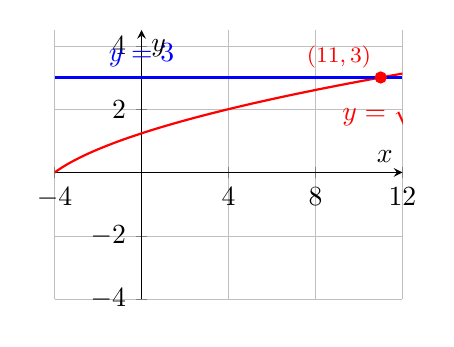
\begin{tikzpicture}
\begin{axis}[
    width=6cm, height=5cm,
    axis lines=middle,
    xmin=-4, xmax=12,
    ymin=-4, ymax=4.5,
    xtick={-4,4,8,12},
    ytick={-4,-2,2,4},
    grid=both,
    grid style={line width=.1pt, draw=gray!20},
    major grid style={line width=.2pt,draw=gray!50},
    xlabel={$x$}, ylabel={$y$},
]
\addplot[domain=-4:12, samples=100, color=red, thick] {sqrt(x+5)-1} node[below right, pos=0.8] {$y=\sqrt{x+5}-1$};
\addplot[domain=-4:12, color=blue, thick] {3} node[above, pos=0.25] {$y=3$};
\addplot[mark=*, color=red] coordinates {(11,3)} node[above left, font=\footnotesize] {$(11,3)$};
\end{axis}
\end{tikzpicture}
\end{center}

\textbf{B. Solve the radical equation $\sqrt[3]{x} + 2 = 4$.}

\begin{align*}
\sqrt[3]{x} + 2 &= 4 \\
\sqrt[3]{x} &= 2 \quad \text{\te{Cube both sides to eliminate the cube root.}} \\
(\sqrt[3]{x})^3 &= 2^3 \\
x &= 8
\end{align*}

So the solution to the radical equation is $x = 8$.

Check your answer by substituting 8 for $x$ in the original equation:
$\sqrt[3]{8} + 2 = 2 + 2 = 4$
\end{example}

\begin{tryit}{1}
Solve each radical equation. Check your solution by substituting into the given equation or graphing.

\textbf{a.} $\sqrt{x - 2} + 3 = 5$ \quad \answer{$x = 6$}

\textbf{b.} $\sqrt[3]{x - 1} = 2$ \quad \answer{$x = 9$}
\end{tryit}

\clearpage
\textbf{APPLICATION}

\begin{example}{2}
\textbf{Rewrite a Formula}

The suspension cables from the Golden Gate Bridge's towers are farther above the roadway near the towers and closer to the roadway near the middle of the bridge. You can figure out your distance from the middle of the bridge, $x$, in feet, and the height of the suspension cable, $y$, in feet, by using the given equation. About how far is the cable from the roadway when you are $200\text{ ft}$ from the middle of the bridge?

\placeholder{photo}{Golden Gate Bridge with the equation $x = \frac{\sqrt{y - 220}}{0.010583}$ pointing to the suspension cable.}

Rewrite the equation to isolate $y$ so you can express the vertical distance between the roadway of the bridge and the suspension cable in terms of $x$.

\begin{align*}
x &= \frac{\sqrt{y - 220}}{0.010583} \\
0.010583x &= \sqrt{y - 220} \\
(0.010583x)^2 &= (\sqrt{y - 220})^2 \\
0.000112x^2 &\approx y - 220 \\
0.000112x^2 + 220 &\approx y \quad \text{\te{This equation gives the vertical distance between the deck and the suspension cable for different values of $x$.}} \\
0.000112(200)^2 + 220 &\approx y \\
224.48 &\approx y
\end{align*}

The cable is about $224\text{ ft}$ above the bridge's roadway when you are $200\text{ ft}$ from the middle of the bridge.
\end{example}

\begin{concept-box}
\textbf{COMMON ERROR}
When squaring a term that includes a coefficient and a variable, remember to square both parts of the term. If you have to round the coefficient after squaring, be sure to use the approximately equal sign.
\end{concept-box}

\begin{tryit}{2}
The speed, $v$, of a vehicle in relation to its stopping distance, $d$, is represented by the equation $v = 3.57\sqrt{d}$. What is the equation for the stopping distance in terms of the vehicle's speed?
\answer{$d = \left(\frac{v}{3.57}\right)^2$}
\end{tryit}

\clearpage
\textbf{CONCEPTUAL UNDERSTANDING}

\begin{example}{3}
\textbf{Identify an Extraneous Solution}

\textbf{A. Solve the radical equation $\sqrt{3x - 2} = x - 4$.}

\begin{align*}
\sqrt{3x - 2} &= x - 4 \\
(\sqrt{3x - 2})^2 &= (x - 4)^2 \\
3x - 2 &= x^2 - 8x + 16 \\
0 &= x^2 - 11x + 18 \\
0 &= (x - 9)(x - 2) \\
x = 9 \quad &\text{or} \quad x = 2
\end{align*}

Check the potential solutions by substituting the solutions for $x$ in the original equation:

\begin{align*}
\sqrt{3x - 2} &= x - 4 & \sqrt{3x - 2} &= x - 4 \\
\sqrt{3(9) - 2} &= 9 - 4 & \sqrt{3(2) - 2} &= 2 - 4 \\
\sqrt{25} &= 5 \ \text{\textcolor{green}{\checkmark}} & \sqrt{4} &\neq -2 \ \text{\textcolor{red}{\ding{55}}}
\end{align*}

So 9 is the only solution to the equation and 2 is an extraneous solution.

\textbf{B. Why does this extraneous solution arise?}

The first step in solving the equation in part (a) was to square both sides. 

Graph on one grid, $y = \sqrt{3x - 2}$ and $y = x - 4$. Then graph on another grid $y = 3x - 2$ and $y = (x - 4)^2$.

\begin{center}
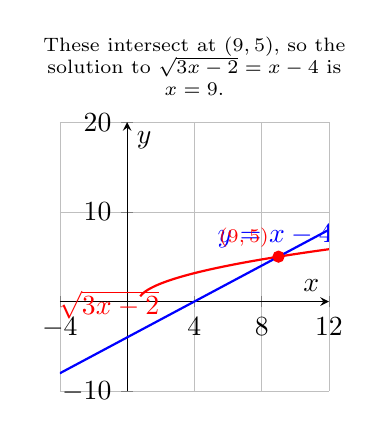
\begin{tikzpicture}
\begin{axis}[
    width=5cm, height=5cm,
    axis lines=middle,
    xmin=-4, xmax=12,
    ymin=-10, ymax=20,
    xtick={-4,4,8,12},
    ytick={-10,10,20},
    grid=both,
    grid style={line width=.1pt, draw=gray!20},
    major grid style={line width=.2pt,draw=gray!50},
    xlabel={$x$}, ylabel={$y$},
    title={\parbox{4cm}{\centering \scriptsize These intersect at $(9, 5)$, so the solution to $\sqrt{3x - 2} = x - 4$ is $x = 9$.}}
]
\addplot[domain=2/3:12, samples=100, color=red, thick] {sqrt(3*x-2)} node[below left, pos=0.2] {$y=\sqrt{3x-2}$};
\addplot[domain=-4:12, color=blue, thick] {x-4} node[above, pos=0.8] {$y=x-4$};
\addplot[mark=*, color=red] coordinates {(9,5)} node[above left, font=\scriptsize] {$(9,5)$};
\end{axis}
\end{tikzpicture}
\quad
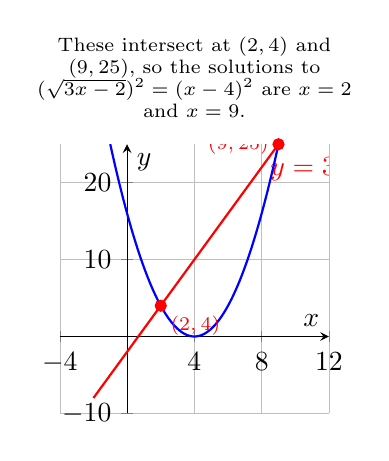
\begin{tikzpicture}
\begin{axis}[
    width=5cm, height=5cm,
    axis lines=middle,
    xmin=-4, xmax=12,
    ymin=-10, ymax=25,
    xtick={-4,4,8,12},
    ytick={-10,10,20},
    grid=both,
    grid style={line width=.1pt, draw=gray!20},
    major grid style={line width=.2pt,draw=gray!50},
    xlabel={$x$}, ylabel={$y$},
    title={\parbox{4cm}{\centering \scriptsize These intersect at $(2, 4)$ and $(9, 25)$, so the solutions to $(\sqrt{3x - 2})^2 = (x - 4)^2$ are $x = 2$ and $x = 9$.}}
]
\addplot[domain=-2:9, color=red, thick] {3*x-2} node[right, pos=0.9] {$y=3x-2$};
\addplot[domain=-1:10, samples=100, color=blue, thick] {(x-4)^2} node[right, pos=0.9] {$y=(x-4)^2$};
\addplot[mark=*, color=red] coordinates {(9,25)} node[left, font=\scriptsize] {$(9,25)$};
\addplot[mark=*, color=red] coordinates {(2,4)} node[below right, font=\scriptsize] {$(2,4)$};
\end{axis}
\end{tikzpicture}
\end{center}

This means that the equations $\sqrt{3x - 2} = x - 4$ and $(\sqrt{3x - 2})^2 = (x - 4)^2$ are not equivalent equations. Both graphs have an intersection point at $x = 9$, but the second graph also has an intersection point at $x = 2$. Squaring both sides of the original equation created an extraneous solution.
\end{example}

\begin{concept-box}
\textbf{VOCABULARY}
An \textbf{extraneous solution} is a solution of an equation derived from an equation, but it is \textit{not} a solution of the original equation.
\end{concept-box}

\begin{tryit}{3}
Solve each radical equation. Check for any extraneous solutions.

\textbf{a.} $x = \sqrt{7x + 8}$ \quad \answer{$x = 8$}

\textbf{b.} $x + 2 = \sqrt{x + 2}$ \quad \answer{$x = -1, -2$}
\end{tryit}

\clearpage

\begin{example}{4}
\textbf{Solve Equations With Rational Exponents}

\textbf{A. What are the solutions to the equation $(x^2 + 5x + 5)^{5/2} = 1$?}

\begin{align*}
(x^2 + 5x + 5)^{5/2} &= 1 \\
((x^2 + 5x + 5)^{5/2})^{2/5} &= (1)^{2/5} \quad \text{\te{Raise both sides to the reciprocal power.}} \\
x^2 + 5x + 5 &= 1 \\
x^2 + 5x + 4 &= 0 \\
(x + 4)(x + 1) &= 0 \quad \text{\te{Use the Zero-Product Property.}} \\
x + 4 = 0 \quad &\text{or} \quad x + 1 = 0 \\
x = -4 \quad &\text{or} \quad x = -1
\end{align*}

Check for extraneous solutions.
\begin{align*}
((-4)^2 + 5(-4) + 5)^{5/2} &\stackrel{?}{=} 1 & ((-1)^2 + 5(-1) + 5)^{5/2} &\stackrel{?}{=} 1 \\
(16 - 20 + 5)^{5/2} &\stackrel{?}{=} 1 & (1 - 5 + 5)^{5/2} &\stackrel{?}{=} 1 \\
(1)^{5/2} &\stackrel{?}{=} 1 & (1)^{5/2} &\stackrel{?}{=} 1 \\
1 &= 1 \ \text{\textcolor{green}{\checkmark}} & 1 &= 1 \ \text{\textcolor{green}{\checkmark}}
\end{align*}

This equation has two solutions, $x = -4$ and $x = -1$. There are no extraneous solutions.

\textbf{B. What is the solution to $(x + 18)^{3/2} = (x - 2)^3$?}

\begin{align*}
(x + 18)^{3/2} &= (x - 2)^3 \\
((x + 18)^{3/2})^{2/3} &= ((x - 2)^3)^{2/3} \quad \text{\te{Raise both sides to the reciprocal power.}} \\
x + 18 &= (x - 2)^2 \\
x + 18 &= x^2 - 4x + 4 \\
x^2 - 5x - 14 &= 0 \\
(x + 2)(x - 7) &= 0 \quad \text{\te{Use the Zero-Product Property.}} \\
x + 2 = 0 \quad &\text{or} \quad x - 7 = 0 \\
x = -2 \quad &\text{or} \quad x = 7
\end{align*}

Check for extraneous solutions.
\begin{align*}
(-2 + 18)^{3/2} &\stackrel{?}{=} (-2 - 2)^3 & (7 + 18)^{3/2} &\stackrel{?}{=} (7 - 2)^3 \\
16^{3/2} &\stackrel{?}{=} (-4)^3 & 25^{3/2} &\stackrel{?}{=} 5^3 \\
64 &\neq -64 \ \text{\textcolor{red}{\ding{55}}} & 125 &= 125 \ \text{\textcolor{green}{\checkmark}}
\end{align*}

So 7 is the only solution to the equation, and -2 is an extraneous solution.
\end{example}

\begin{concept-box}
\textbf{STUDY TIP}
An equation can have one solution, multiple solutions, or no solutions, so it's important to check all potential solutions.
\end{concept-box}

\begin{tryit}{4}
Solve each equation.

\textbf{a.} $(x^2 - 3x - 6)^{3/2} - 14 = -6$ \quad \answer{$x = 10, -7$}

\textbf{b.} $(x - 8)^{3/2} = (10 - x)^3$ \quad \answer{$x = 9$}
\end{tryit}

\clearpage

\begin{example}{5}
\textbf{Solve an Equation With Two Radicals}

\textbf{Solve the radical equation $\sqrt{x + 9} - \sqrt{2x} = 3$.}

When an equation has two radicals, start the solution process by isolating one radical.

\begin{align*}
\sqrt{x + 9} - \sqrt{2x} &= 3 \\
\sqrt{x + 9} &= \sqrt{2x} + 3 \quad \text{\te{Isolate one radical sign.}} \\
(\sqrt{x + 9})^2 &= (\sqrt{2x} + 3)^2 \\
x + 9 &= 2x + 6\sqrt{2x} + 9 \\
0 &= x + 6\sqrt{2x} \\
-x &= 6\sqrt{2x} \quad \text{\te{Isolate the remaining radical and square again.}} \\
(-x)^2 &= (6\sqrt{2x})^2 \\
x^2 - 72x &= 0 \\
x(x - 72) &= 0 \\
x = 0 \quad &\text{or} \quad x = 72
\end{align*}

Check the potential solutions by substituting 0 and 72 for $x$ in the original equation:

\begin{align*}
\sqrt{x + 9} - \sqrt{2x} &\stackrel{?}{=} 3 & \sqrt{x + 9} - \sqrt{2x} &\stackrel{?}{=} 3 \\
\sqrt{(0) + 9} - \sqrt{2(0)} &\stackrel{?}{=} 3 & \sqrt{(72) + 9} - \sqrt{2(72)} &\stackrel{?}{=} 3 \\
\sqrt{9} - \sqrt{0} &\stackrel{?}{=} 3 & \sqrt{81} - \sqrt{144} &\stackrel{?}{=} 3 \\
3 - 0 &\stackrel{?}{=} 3 & 9 - 12 &\stackrel{?}{=} 3 \\
3 &= 3 \ \text{\textcolor{green}{\checkmark}} & -3 &\neq 3 \ \text{\textcolor{red}{\ding{55}}}
\end{align*}

The only solution is $0$. The value $72$ does not make the original equation true, so it is an extraneous solution.

You can also see this by graphing $y = \sqrt{x + 9} - \sqrt{2x}$ and $y = 3$ together. They intersect only at $x = 0$.

\begin{center}
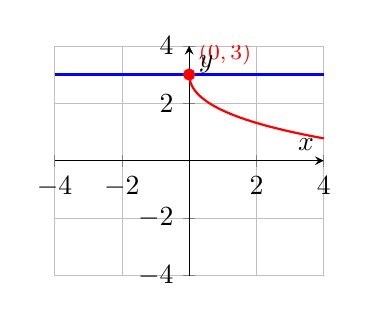
\begin{tikzpicture}
\begin{axis}[
    width=5cm, height=4.5cm,
    axis lines=middle,
    xmin=-4, xmax=4,
    ymin=-4, ymax=4,
    xtick={-4,-2,2,4},
    ytick={-4,-2,2,4},
    grid=both,
    grid style={line width=.1pt, draw=gray!20},
    major grid style={line width=.2pt,draw=gray!50},
    xlabel={$x$}, ylabel={$y$},
]
\addplot[domain=0:4, samples=100, color=red, thick] {sqrt(x+9)-sqrt(2*x)};
\addplot[domain=-4:4, color=blue, thick] {3};
\addplot[mark=*, color=red] coordinates {(0,3)} node[above right, font=\footnotesize] {$(0,3)$};
\end{axis}
\end{tikzpicture}
\end{center}
\end{example}

\begin{concept-box}
\textbf{COMMON ERROR}
A common mistake when squaring an expression like $\sqrt{2x} + 3$ is to only square the radical portion. Square this expression as you would any binomial, by using the Distributive Property.
\end{concept-box}

\begin{tryit}{5}
Solve each radical equation. Check for extraneous solutions.

\textbf{a.} $\sqrt{x + 4} - \sqrt{3x} = -2$ \quad \answer{$x = 12$}

\textbf{b.} $\sqrt{15 - x} - \sqrt{6x} = -3$ \quad \answer{$x = 6$}
\end{tryit}

\clearpage
\textbf{APPLICATION}

\begin{example}{6}
\textbf{Solve a Radical Inequality}

The body surface area (BSA) of a human being is used to determine some doses of medication. The formula for finding BSA is $BSA = \sqrt{\frac{H \cdot M}{3,600}}$, where $H$ is the height in centimeters and $M$ is the mass in kilograms.

A doctor calculates a particular dose of medicine for a patient. What must the mass of the person be for the dose to be appropriate?

\placeholder{illustration}{A doctor looking at a tablet. The tablet shows: $BSA < 1.9$, $Height = 160\text{cm}$.}

\begin{align*}
BSA &< 1.9 \\
\sqrt{\frac{H \cdot M}{3,600}} &< 1.9 \quad \text{\te{Substitute in an expression equal to $BSA$.}} \\
\sqrt{\frac{160 \cdot M}{3,600}} &< 1.9 \quad \text{\te{Substitute 160 for $H$, and solve for $M$.}} \\
\left(\sqrt{\frac{160 \cdot M}{3,600}}\right)^2 &< 1.9^2 \\
\frac{160 \cdot M}{3,600} &< 3.61 \\
M &< 81.225
\end{align*}

The mass of the patient must be less than $81.225\text{ kg}$ for the dose to be appropriate.
\end{example}

\begin{concept-box}
\textbf{CONSTRUCT ARGUMENTS}
Another way to solve this problem is to substitute values into the formula, solve it as an equation, and then use logic to determine the inequality symbol. When there are many possible solution methods, how do you decide which to use?
\end{concept-box}

\begin{tryit}{6}
A doctor calculates that a particular dose of medicine is appropriate for an individual whose BSA is less than $1.8$. If the mass of the individual is $75\text{ kg}$, how many cm tall can he or she be for the dose to be appropriate?
\answer{$H < 155.52\text{ cm}$}
\end{tryit}

\clearpage

\begin{concept-summary}
\textbf{Solving Radical Equations}

\begin{tabular}{p{1.5cm} p{3.5cm} p{4cm} p{4cm}}
\toprule
 & \textbf{WORDS} & \textbf{ALGEBRA} & \textbf{GRAPH} \\
\midrule
\textbf{Step 1} & Isolate the radical term. & $2\sqrt{x + 3} - x = 0$ \newline $2\sqrt{x + 3} = x$ & \multirow{4}{*}{
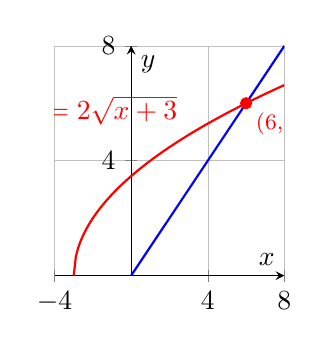
\begin{tikzpicture}[baseline=(current bounding box.center)]
\begin{axis}[
    width=4.5cm, height=4.5cm,
    axis lines=middle,
    xmin=-4, xmax=8,
    ymin=0, ymax=8,
    xtick={-4,0,4,8},
    ytick={4,8},
    grid=both,
    grid style={line width=.1pt, draw=gray!20},
    major grid style={line width=.2pt,draw=gray!50},
    xlabel={$x$}, ylabel={$y$},
]
\addplot[domain=-3:8, samples=100, color=red, thick] {2*sqrt(x+3)} node[above left, pos=0.6] {$y=2\sqrt{x+3}$};
\addplot[domain=-4:8, color=blue, thick] {x} node[above] {$y=x$};
\addplot[mark=*, color=red] coordinates {(6,6)} node[below right, font=\footnotesize] {$(6,6)$};
\end{axis}
\end{tikzpicture}
} \\
\textbf{Step 2} & Square both sides to remove the radical. & $(2\sqrt{x + 3})^2 = (x)^2$ & \\
\textbf{Step 3} & Solve the equation. & $4(x + 3) = x^2$ \newline $x^2 - 4x - 12 = 0$ \newline $(x - 6)(x + 2) = 0$ \newline $x = 6 \text{ or } x = -2$ & \\
\textbf{Step 4} & Eliminate extraneous solutions. & $2\sqrt{6 + 3} - 6 \stackrel{?}{=} 0$ \newline $2\sqrt{9} \stackrel{?}{=} 6$ \newline $6 \stackrel{?}{=} 6$ \newline $6 = 6 \ \text{\textcolor{green}{\checkmark}}$ \newline\newline $2\sqrt{-2 + 3} - (-2) \stackrel{?}{=} 0$ \newline $2\sqrt{1} \stackrel{?}{=} -2$ \newline $2 \stackrel{?}{=} -2$ \newline $2 \neq -2 \ \text{\textcolor{red}{\ding{55}}}$ & \\
\bottomrule
\end{tabular}
\end{concept-summary}

\vspace{1em}

\begin{minipage}[t]{0.45\textwidth}
\textbf{\large Do You UNDERSTAND?}

\begin{practice}{1}{}
\textbf{ESSENTIAL QUESTION} What properties of exponents allow you to solve equations that include radicals or rational exponents?
\end{practice}

\begin{practice}{2}{}
\textbf{Construct Arguments} How can you use a graph to show that the solution to $\sqrt[3]{84x + 8} = 8$ is 6?
\end{practice}

\begin{practice}{3}{}
\textbf{Vocabulary} Why does solving a radical equation sometimes result in an extraneous solution?
\end{practice}

\begin{practice}{4}{}
\textbf{Error Analysis} Nazim said that $-3$ and $6$ are the solutions to $\sqrt{3x + 18} = x$. What error did Nazim make?
\end{practice}

\begin{practice}{5}{}
\textbf{Communicate Precisely} Describe how you would solve the equation $x^{2/3} = n$. How is this solution method to be interpreted if the equation had been written in radical form instead?
\end{practice}
\end{minipage}
\hfill
\begin{minipage}[t]{0.5\textwidth}
\textbf{\large Do You KNOW HOW?}

Solve for $x$.

\begin{practice}{6}{}
$3\sqrt{x} + 22 = 21$
\end{practice}

\begin{practice}{7}{}
$\sqrt[3]{5x} = 25$
\end{practice}

In 8 and 9, find the extraneous solution.

\begin{practice}{8}{}
$\sqrt{8x + 9} = x$
\end{practice}

\begin{practice}{9}{}
$x = \sqrt{24 - 2x}$
\end{practice}

\begin{practice}{10}{}
Rewrite the equation $y = \sqrt{\frac{x - 48}{6}}$ to isolate $x$.
\end{practice}

\begin{practice}{11}{}
Use a graph to find the solution to the equation $9 = \sqrt{3x + 11}$.
\end{practice}

Solve each equation.

\begin{practice}{12}{}
$(3x + 2)^{2/3} = 4$
\end{practice}

\begin{practice}{13}{}
$\sqrt{2x - 5} - \sqrt{x - 3} = 1$
\end{practice}

\begin{practice}{14}{}
$\sqrt{x + 2} + \sqrt{3x + 4} = 2$
\end{practice}
\end{minipage}

\clearpage

\textbf{\Large PRACTICE \& PROBLEM SOLVING}

\begin{minipage}[t]{0.45\textwidth}
\textbf{\large UNDERSTAND}

\begin{practice}{15}{}
\textbf{Generalize} Explain how to identify an extraneous solution for an equation containing a radical expression.
\end{practice}

\begin{practice}{16}{}
\textbf{Look for Relationships} Write a radical equation that relates a square's perimeter to its area. Explain your reasoning. Use $s$ to represent the side length of the square.
\end{practice}

\begin{practice}{17}{}
\textbf{Error Analysis} Describe and correct the error a student made in rewriting the equation to isolate $y$.

\begin{center}
\colorbox{gray!10}{\parbox{4cm}{
\begin{align*}
x &= \frac{\sqrt{58 + y}}{1.98} \\
1.98x &= \sqrt{58 + y} \\
1.98x^2 &= 58 + y \quad \text{\textcolor{red}{\ding{55}}} \\
1.98x^2 - 58 &= y
\end{align*}
}}
\end{center}
\end{practice}

\begin{practice}{18}{}
\textbf{Use Appropriate Tools} Find the point of intersection of the two graphs.

\begin{center}
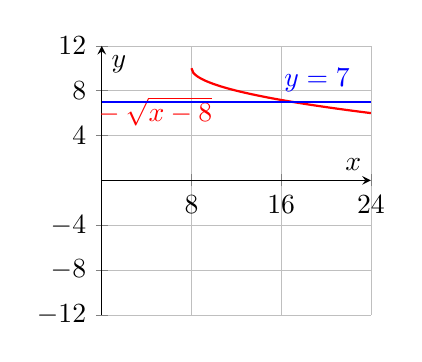
\begin{tikzpicture}
\begin{axis}[
    width=5cm, height=5cm,
    axis lines=middle,
    xmin=0, xmax=24,
    ymin=-12, ymax=12,
    xtick={8,16,24},
    ytick={-12,-8,-4,4,8,12},
    grid=both,
    grid style={line width=.1pt, draw=gray!20},
    major grid style={line width=.2pt,draw=gray!50},
    xlabel={$x$}, ylabel={$y$},
]
\addplot[domain=8:24, samples=100, color=red, thick] {10-sqrt(x-8)} node[below left, pos=0.2] {$y=10-\sqrt{x-8}$};
\addplot[domain=0:24, color=blue, thick] {7} node[above, pos=0.8] {$y=7$};
\end{axis}
\end{tikzpicture}
\end{center}
\end{practice}

\begin{practice}{19}{}
\textbf{Higher Order Thinking} Some, but not all, equations with rational exponents have extraneous solutions. What is the relationship between the exponents and the possibility of having extraneous solutions for equations with rational exponents? Explain your reasoning.
\end{practice}

\begin{practice}{20}{}
\textbf{Communicate Precisely} Describe the process used to solve an equation with two radical expressions. How is this process different from solving an equation with only one radical expression?
\end{practice}
\end{minipage}
\hfill
\begin{minipage}[t]{0.5\textwidth}
\textbf{\large PRACTICE}

Solve each radical equation. \textsc{SEE EXAMPLE 1}

\begin{practice}{21}{}
$\sqrt[3]{x} + 8 = 13$
\end{practice}

\begin{practice}{22}{}
$\sqrt{4x} = 11$
\end{practice}

\begin{practice}{23}{}
$\sqrt{75 + x} - 6 = 14$
\end{practice}

\begin{practice}{24}{}
$25 - \sqrt[4]{x} = 22$
\end{practice}

Solve for $y$. \textsc{SEE EXAMPLE 2}

\begin{practice}{25}{}
$x = 3(\sqrt[3]{15 + y})$
\end{practice}

\begin{practice}{26}{}
$x = \frac{\sqrt{2y}}{26}$
\end{practice}

\begin{practice}{27}{}
$x = \frac{\sqrt{y - 14.2}}{0.05}$
\end{practice}

\begin{practice}{28}{}
$x = \frac{1}{3}(\sqrt[4]{y})$
\end{practice}

Solve each radical equation. Check for extraneous solutions. \textsc{SEE EXAMPLE 3}

\begin{practice}{29}{}
$x = \sqrt{x + 6}$
\end{practice}

\begin{practice}{30}{}
$2x = \sqrt{17x - 15}$
\end{practice}

\begin{practice}{31}{}
$4x = \sqrt{6x + 10}$
\end{practice}

\begin{practice}{32}{}
$x = \sqrt{56 - x}$
\end{practice}

Solve. \textsc{SEE EXAMPLE 4}

\begin{practice}{33}{}
$0.5(x^2 + 5x + 136)^{2/3} = 50$
\end{practice}

\begin{practice}{34}{}
$2(x^2 - 12x - 4)^{1/2} - 3 = 15$
\end{practice}

\begin{practice}{35}{}
$(x^2 + 4x + 5)^{3/2} + 1 = 0$
\end{practice}

Solve each radical equation. Check for extraneous solutions. \textsc{SEE EXAMPLE 5}

\begin{practice}{36}{}
$\sqrt{6 + x} - \sqrt{x - 5} = 2$
\end{practice}

\begin{practice}{37}{}
$\sqrt{4x + 5} - \sqrt{x + 1} = 1$
\end{practice}

\begin{practice}{38}{}
$\sqrt{x + 1} + 1 = \sqrt{x + 3}$
\end{practice}

Solve using the formula $BSA = \sqrt{\frac{H \cdot M}{3,600}}$. \textsc{SEE EXAMPLE 6}

\begin{practice}{39}{}
A sports medicine specialist determines that a hot-weather training strategy is appropriate for this athlete. To the nearest tenth, what can the mass of the athlete be for the training strategy to be appropriate?

\placeholder{illustration}{A female runner finishing a race. Labels point to her: "Finish", bib number "1789", height "165 cm", and a note "BSA < 2.0".}
\end{practice}
\end{minipage}

\clearpage

\begin{minipage}[t]{0.45\textwidth}
\textbf{\large APPLY}

\begin{practice}{40}{}
Specialists can determine the speed a vehicle was traveling from the length of its skid marks, $d$, and the coefficient of friction, $f$. Rewrite the formula to solve for the length of the skid marks.

\placeholder{illustration}{A car leaving skid marks on a curvy road. A text box says: "Vehicle's speed is $15.9\sqrt{df}$."}
\end{practice}

\begin{practice}{41}{}
\textbf{Make Sense and Persevere} The half-life of a certain type of soft drink is $5\text{ h}$. If you drink $50\text{ mL}$ of this drink, the formula $y = 50(0.5)^{t/5}$ tells the amount of the drink left in your system after $t$ hours. How much of the soft drink will be left in your system after 16 hours?
\end{practice}

\begin{practice}{42}{}
\textbf{Model With Mathematics} Big Ben's pendulum takes $4\text{ s}$ to swing back and forth. The formula $t = 2\pi\sqrt{\frac{L}{32}}$ gives the swing time, $t$, in seconds, based on the length of the pendulum, $L$, in feet. What is the minimum length necessary to build a clock with a pendulum that takes longer than Big Ben's pendulum to swing back and forth?
\end{practice}

\begin{practice}{43}{}
\textbf{Make Sense and Persevere} Derek is hang gliding on a clear day. Use the formula for visibility, $v = 1.225\sqrt{a}$ to find the altitude at which Derek is hang gliding.

\placeholder{illustration}{A person hang gliding. Labels say: "visibility, $v = 67.1$ miles" and "Distance to ground = $a$ feet".}
\end{practice}
\end{minipage}
\hfill
\begin{minipage}[t]{0.5\textwidth}
\textbf{\large ASSESSMENT PRACTICE}

\begin{practice}{44}{}
Complete the table to solve for the unknown value in the equation $y = \sqrt[3]{2x + z} - 12$, using the given values in each row.

\begin{center}
\begin{tabular}{|c|c|c|}
\hline
\textbf{$y$} & \textbf{$x$} & \textbf{$z$} \\
\hline
0 & 462 & \\
\hline
$-3$ & & 439 \\
\hline
$-10$ & 1.25 & \\
\hline
3 & & 16 \\
\hline
\end{tabular}
\end{center}
\end{practice}

\begin{practice}{45}{}
\textbf{SAT/ACT} What is the solution to the equation $(x^2 + 5x + 25)^{3/2} = 343$?

\begin{itemize}
    \item[A] $-8$ only
    \item[B] 3 only
    \item[C] 77 only
    \item[D] $-8$ and 3
    \item[E] There are no solutions.
\end{itemize}
\end{practice}

\begin{practice}{46}{}
\textbf{Performance Task} Escape velocity is the velocity at which an object must be traveling to leave a star or planet without falling back to its surface or into orbit. Escape velocity depends on the gravitational constant, $G = 6.67 \times 10^{-11}$, the mass, $M$ in kilograms, and radius, $r$, of the star or planet.

\placeholder{illustration}{Earth with a rocket trajectory illustrating escape velocity. Labels: "Escape velocity: $v = \sqrt{\frac{2GM}{r}}$" and "Earth's radius = 6,371,000 m".}

\textbf{Part A} Rewrite the equation to solve for mass.

\textbf{Part B} Earth has an escape velocity of about $11,200$ meters per second. What is Earth's mass in kilograms?
\end{practice}
\end{minipage}

\clearpage

\textbf{\Large MATHEMATICAL MODELING IN 3 ACTS}

\textbf{\LARGE The Snack Shack}

Americans seem to love the beach! When the weather is warm, people flock to the beach. Some people bring coolers packed with food and drinks. Others prefer to take advantage of snack bars and shops set up along the beach.

Some beachside communities have built long wooden walkways, or boardwalks, to make it easier for beachgoers to walk to the snack bars and stores. How easy do you find walking in the sand? Think about this during the Mathematical Modeling in 3 Acts lesson.

\placeholder{photo}{A wooden boardwalk extending over a sandy beach toward distant mountains.}

\vspace{1em}

\colorbox{blue!80}{\textcolor{white}{\textbf{ACT 1}}} \quad \textbf{Identify the Problem}

\begin{enumerate}
    \item What is the first question that comes to mind after watching the video?
    \item Write down the main question you will answer about what you saw in the video.
    \item Make an initial conjecture that answers this main question.
    \item Explain how you arrived at your conjecture.
    \item What information will be useful to know to answer the main question? How can you get it? How will you use that information?
\end{enumerate}

\vspace{1em}

\colorbox{blue!80}{\textcolor{white}{\textbf{ACT 2}}} \quad \textbf{Develop a Model}

\begin{enumerate}
    \setcounter{enumi}{5}
    \item Use the math that you have learned in this Topic to refine your conjecture.
\end{enumerate}

\vspace{1em}

\colorbox{blue!80}{\textcolor{white}{\textbf{ACT 3}}} \quad \textbf{Interpret the Results}

\begin{enumerate}
    \setcounter{enumi}{6}
    \item Did your refined conjecture match the actual answer exactly? If not, what might explain the difference?
\end{enumerate}

\end{document}